%-------------------------------------------------------------------------------

% This file is part of Code_Saturne, a general-purpose CFD tool.
%
% Copyright (C) 1998-2011 EDF S.A.
%
% This program is free software; you can redistribute it and/or modify it under
% the terms of the GNU General Public License as published by the Free Software
% Foundation; either version 2 of the License, or (at your option) any later
% version.
%
% This program is distributed in the hope that it will be useful, but WITHOUT
% ANY WARRANTY; without even the implied warranty of MERCHANTABILITY or FITNESS
% FOR A PARTICULAR PURPOSE.  See the GNU General Public License for more
% details.
%
% You should have received a copy of the GNU General Public License along with
% this program; if not, write to the Free Software Foundation, Inc., 51 Franklin
% Street, Fifth Floor, Boston, MA 02110-1301, USA.

%-------------------------------------------------------------------------------

\programme{itrmas/itrgrp}

\vspace{1cm}
%%%%%%%%%%%%%%%%%%%%%%%%%%%%%%%%%%
%%%%%%%%%%%%%%%%%%%%%%%%%%%%%%%%%%
\section*{Fonction}
%%%%%%%%%%%%%%%%%%%%%%%%%%%%%%%%%%
%%%%%%%%%%%%%%%%%%%%%%%%%%%%%%%%%%
Le but du sous-programme \fort{itrmas} est de calculer un gradient de pression
``facette''. Il est utilis\'e dans la phase de correction de pression
(deuxi\`eme phase de \fort{navsto}) o\`u le flux de masse est mis \`a jour \`a l'aide de termes en $-\Delta t_{\,ij}(\grad_f P)_{\,ij}.\vect{S}_{\,ij}$ et en $-\Delta t_{\,b_{ik}}(\grad_f P)_{\,b_{ik}}\,.\,\vect{S}_{\,b_{ik}}$.

Le sous-programme \fort{itrgrp} calcule un gradient ``facette'' de pression et
en prend la divergence, c'est-\`a-dire calcule le terme :
\begin{displaymath}
-\sum\limits_{j\in Vois(i)}\Delta t_{\,ij}(\grad_f P)_{\,ij}.\vect{S}_{\,ij}
-\sum\limits_{k\in\gamma_b(i)}\Delta t_{\,b_{ik}}(\grad_f P)_{\,b_{ik}}\,.\,\vect{S}_{\,b_{ik}}
\end{displaymath}
En pratique \fort{itrgrp} correspond \`a la combinaison de \fort{itrmas} et de
\fort{divmas}, mais permet par son traitement en un seul bloc d'\'eviter la
d\'efinition de tableaux de travail de taille \var{NFAC} et \var{NFABOR}.

%%%%%%%%%%%%%%%%%%%%%%%%%%%%%%%%%%
%%%%%%%%%%%%%%%%%%%%%%%%%%%%%%%%%%
\section*{Discr\'etisation}
%%%%%%%%%%%%%%%%%%%%%%%%%%%%%%%%%%
%%%%%%%%%%%%%%%%%%%%%%%%%%%%%%%%%%

La figure \ref{Base_Itrmas_fig_geom} rappelle les diverses d\'efinitions g\'eom\'etriques
pour les faces internes et les faces de bord.

\begin{figure}[h]
\parbox{8cm}{%
\centerline{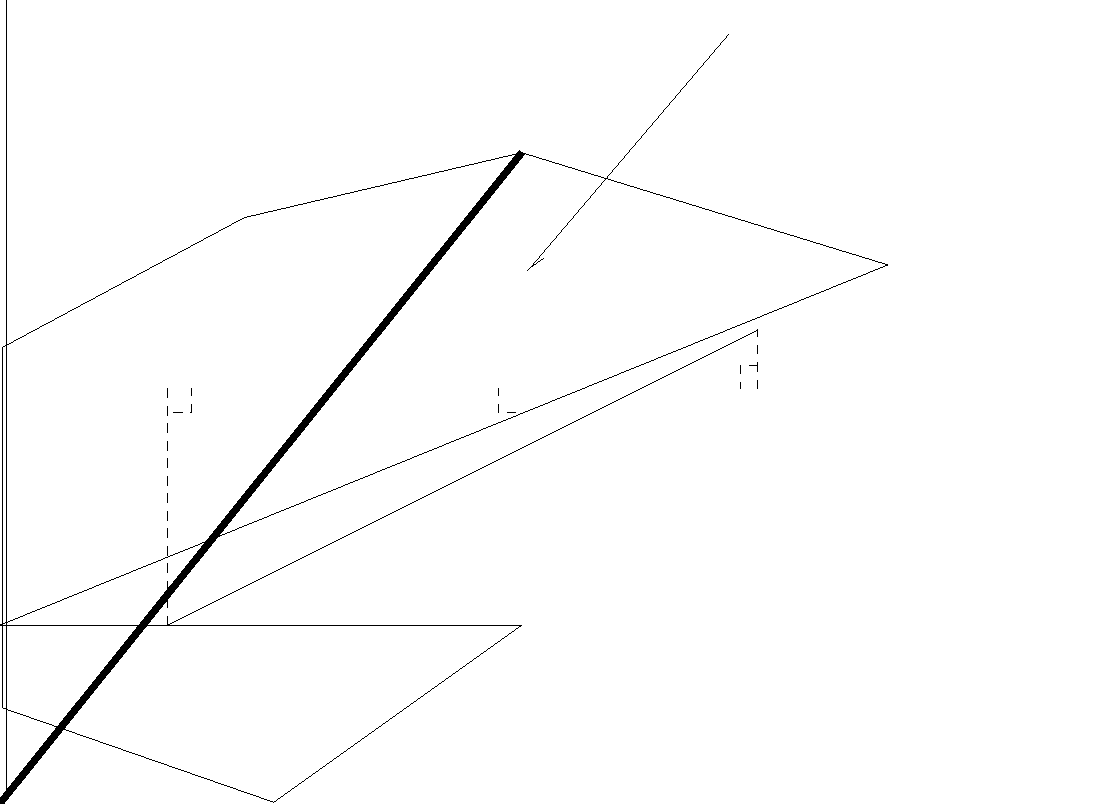
\includegraphics[height=4cm]{facette}}}
\parbox{8cm}{%
\centerline{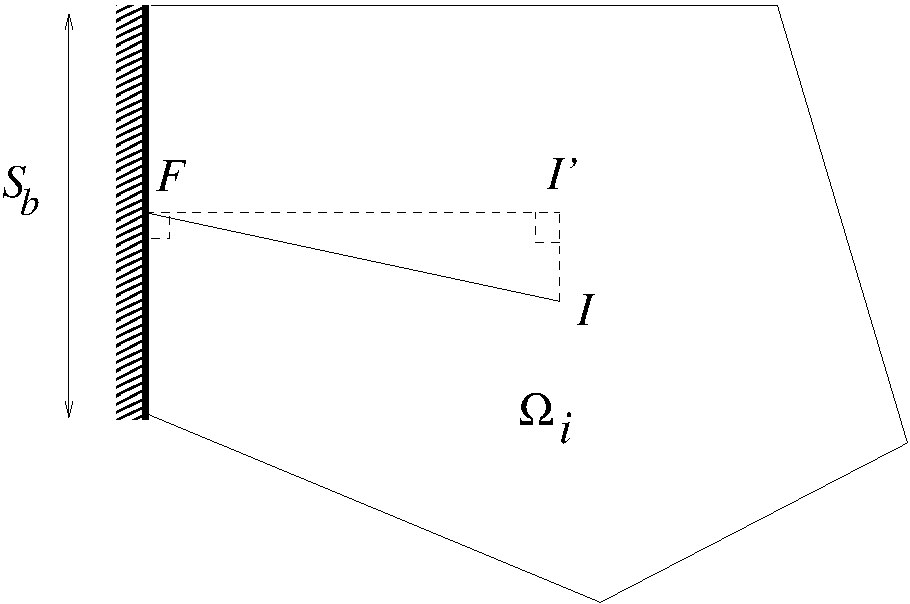
\includegraphics[height=4cm]{facebord}}}
\caption{\label{Base_Itrmas_fig_geom}D\'efinition des diff\'erentes entit\'es
g\'eom\'etriques pour les faces internes (gauche) et de bord (droite).}
\end{figure}


\subsection*{Calcul sans reconstruction des non orthogonalit\'es}
Pour les faces internes, on \'ecrit simplement :
\begin{equation}
\label{Base_Itrmas_eq_intssrec}
-\Delta t_{\,ij}(\grad_f P)_{\,ij}\,.\,\vect{S}_{\,ij}=
\frac{\Delta t_{\,ij}S_{\,ij}}{\overline{I^\prime J^\prime}}(P_I-P_J)
\end{equation}

Pour les faces de bord, on \'ecrit :
\begin{equation}
\label{Base_Itrmas_eq_brdssrec}
-\Delta t_{b_{ik}}(\grad_f P)_{\,b_{ik}}\,.\,\vect{S}_{\,b_{ik}}=
\frac{\Delta t_{\,b_{ik}}S_{\,b_{ik}}}{\overline{I^\prime F}}
\left((1-B_{b,ik})P_I-\var{INC}\times A_{b,ik}\right)
\end{equation}

Les pas de temps aux faces $\Delta t_{\,ij}$ et $\Delta t_{\,b_{ik}}$ sont calcul\'es
par interpolation par les sous-programmes \fort{viscfa} (cas isotrope,
\var{IPUCOU=0}) ou \fort{visort} (cas anisotrope, \var{IPUCOU=1}).


\subsection*{Calcul avec reconstruction des non orthogonalit\'es}
Plusieurs discr\'etisations peuvent \^etre propos\'ees pour le traitement des
non orthogonalit\'es. Celle retenue dans le code est issue des premiers tests
r\'ealis\'es sur le prototype, et fait intervenir non seulement le pas de temps
interpol\'e \`a la face, mais aussi les pas de temps dans chaque
cellule. Il
serait sans doute bon de revenir sur cette \'ecriture et \'evaluer d'autres
solutions. La forme utilis\'ee pour les faces internes est :
\begin{multline}
\label{Base_Itrmas_eq_intavcrec}
-\Delta t_{\,ij}(\grad_f P)_{\,ij}\,.\,\vect{S}_{\,ij}=
\frac{\Delta t_{\,ij}S_{\,ij}}{\overline{I^\prime J^\prime}}(P_I-P_J)\\
+(\vect{II}^\prime-\vect{JJ}^\prime).\frac{1}{2}\left[
\Delta t_I(\grad P)_I+\Delta t_J(\grad P)_J\right]
\frac{S_{\,ij}}{\overline{I^\prime J^\prime}}
\end{multline}

Pour les faces de bord, on \'ecrit :
\begin{equation}
\label{Base_Itrmas_eq_brdavcrec}
-\Delta t_{\,b_{ik}}(\grad_f P)_{\,b_{ik}}\,.\,\vect{S}_{\,b_{ik}}=
\frac{\Delta t_{\,b_{ik}} S_{\,b_{ik}}}{\overline{I^\prime F}}
\left[(1-B_{b,ik})(P_I+\vect{II}^\prime.(\grad P)_I)-\var{INC}\times A_{b,ik}\right]
\end{equation}

%%%%%%%%%%%%%%%%%%%%%%%%%%%%%%%%%%
%%%%%%%%%%%%%%%%%%%%%%%%%%%%%%%%%%
\section*{Mise en \oe uvre}
%%%%%%%%%%%%%%%%%%%%%%%%%%%%%%%%%%
%%%%%%%%%%%%%%%%%%%%%%%%%%%%%%%%%%
Les principaux arguments pass\'es \`a \fort{itrmas} et \fort{itrgrp} sont la
variable trait\'ee \var{PVAR} (la pression), ses conditions aux limites, le pas
de temps projet\'e aux faces\footnote{%
Plus pr\'ecis\'ement, le pas de temps projet\'e aux faces, multipli\'e par la
surface et divis\'e par $\overline{I^\prime J^\prime}$ ou $\overline{I^\prime F}$, cf. \fort{viscfa}}
(\var{VISCF} et \var{VISCB}), le pas de temps au
centre des cellules, \'eventuellement anisotrope (\var{VISELX}, \var{VISELY},
\var{VISELZ}). \fort{itrmas} retourne les tableaux \var{FLUMAS} et \var{FLUMAB}
(flux de masse aux faces) mis \`a jour. \fort{itrgrp} retourne directement la
divergence du flux de masse mis \`a jour, dans le tableau \var{DIVERG}.

\etape{Initialisation}
Si \var{INIT} vaut 1, les variables \var{FLUMAS} et \var{FLUMAB} ou \var{DIVERG}
sont mises \`a z\'ero.

\etape{Cas sans reconstruction}
La prise en compte ou non des non orthogonalit\'es est d\'etermin\'ee par
l'indicateur \var{NSWRGR} de la variable trait\'ee (nombre de sweeps de
reconstruction des non orthogonalit\'es dans le calcul des gradients), pass\'e
par la variable \var{NSWRGP}. Une valeur inf\'erieure ou \'egale \`a 1 enclenche
le traitement sans reconstruction.\\
Des boucles sur les faces internes et les faces de bord utilisent directement
les formules (\ref{Base_Itrmas_eq_intssrec}) et (\ref{Base_Itrmas_eq_brdssrec}) pour remplir les
tableaux \var{FLUMAS} et \var{FLUMAB} (\fort{itrmas}) ou des variables de
travail \var{FLUMAS} et \var{FLUMAB} qui servent \`a mettre \`a jour le tableau
\var{DIVERG} (\fort{itrgrp}).

\`A noter que les tableaux \var{VISCF} et \var{VISCB} contiennent respectivement
$\displaystyle\frac{\Delta t_{\,ij}S_{\,ij}}{\overline{I^\prime J^\prime}}$ et
$\displaystyle\frac{\Delta t_{\,b_{ik}}S_{\,b_{ik}}}{\overline{I^\prime F}}$.

\etape{Cas avec reconstruction}
Apr\`es un appel \`a \fort{GRDCEL} pour calculer le gradient cellule de
pression, on remplit les tableaux \var{FLUMAS} et \var{FLUMAB} ou \var{DIVERG}
l\`a encore par une application directe des formules (\ref{Base_Itrmas_eq_intavcrec}) et
(\ref{Base_Itrmas_eq_brdavcrec}).

%%%%%%%%%%%%%%%%%%%%%%%%%%%%%%%%%%
%%%%%%%%%%%%%%%%%%%%%%%%%%%%%%%%%%
\section*{Points \`a traiter}
%%%%%%%%%%%%%%%%%%%%%%%%%%%%%%%%%%
%%%%%%%%%%%%%%%%%%%%%%%%%%%%%%%%%%
Il est un peu redondant de passer en argument \`a la fois le pas de temps
projet\'e aux faces et le pas de temps au centre des cellules. Il faudrait
s'assurer de la r\'eelle n\'ecessit\'e de cela, ou alors \'etudier des
formulations plus simples de la partie reconstruction.

